\section{Life Cycle Assessment (LCA)}\label{sec:Background}

Production systems are seen world wide, to provide all the commercial and industrial products demanded by the modern world. These products influence the world we live in, in one way or another. In order to control the environmental impact, these influences have to be considered when such systems are created/maintained. 

These systems exist in a wide variety of sizes and applications, making the systems diverse, and difficult to compare to each other. A general approach is necessary to characterise the production systems, and validate that the systems are sustainable and meet regulations.

Life cycle assessment is an approach to characterise and assess the overall environmental impact of a production system, and throughout the products lifetime.

LCA is becoming increasingly more acknowledged, and has been since the 60’s, as environmental impact and resource depletion have become a great concern. Today's regulations must be met to certify a bounded level of environmental impact throughout a products life cycle. (\cite{LCA_TheoryAndPractice} chapter 1.1)

As an example of a production system, we may look at a simple system producing apple juice. To create this product, we definitely need apples, and means of containing the juice. With just these two necessities, we have to evaluate the resources needed to farm the applies, produce the juice, create the container, deliver the product, dispose of container after use, resulting in machinery, fertiliser, manpower, transport, heating, apple waste etc.. 

\begin{figure}[H]
    \centering
    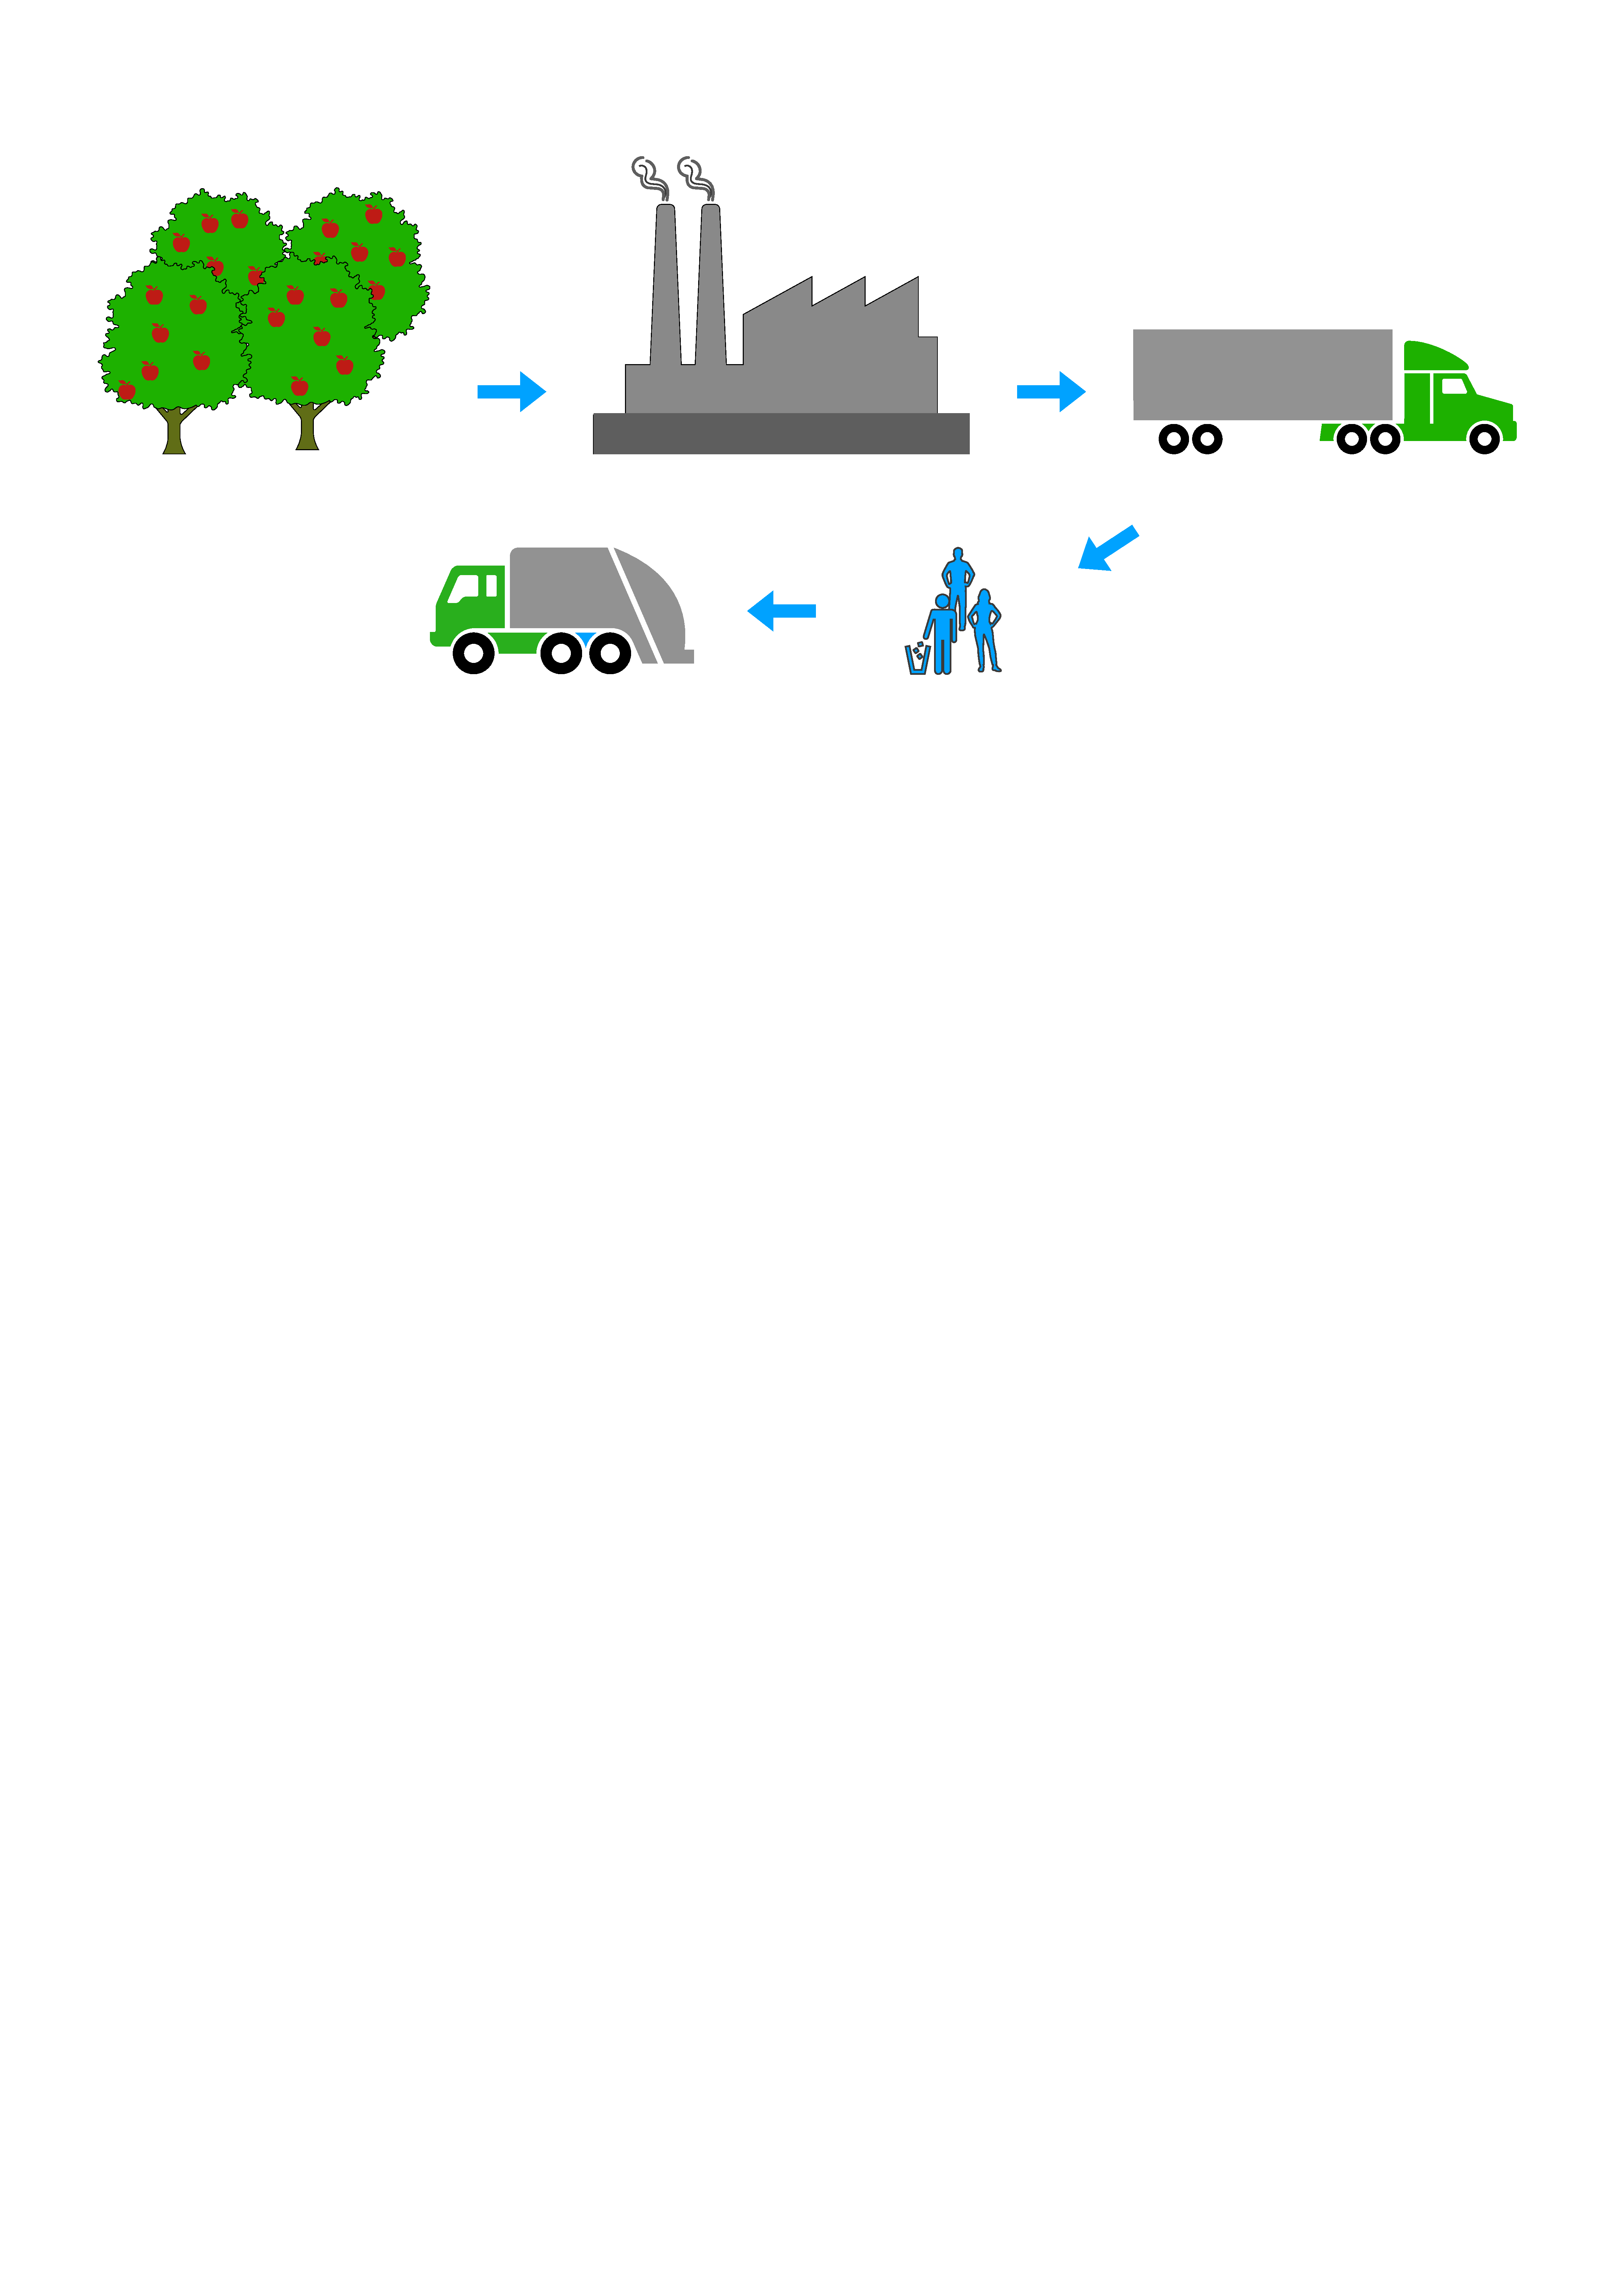
\includegraphics[page=1, width=0.7\linewidth] {.Figures/AppleJuiceExample.pdf}
    \caption{Apple juice life cycle example.}
    \label{fig:lifecycleExample}
\end{figure}

It quickly becomes difficult to evaluate the overall environmental impact, even for such a simple production system. Therefore to evaluate our apple juice production system, we will try to look at how LCA proceeds with such an evaluation.

As we have seen, many factors contribute to the total impact of a production system, and without looking at the complete life cycle of the product, from initial resources, through creation, to disposal or recycling, it is not possible to make a qualified estimate.

Since 1990 the methodologies in LCA have been developed greatly, but for simplicity we will look at the four main phases and hot they relate to the evaluation of our apply juice production. (\cite{LCA_TheoryAndPractice} chapter 6.2)

Throughout the different phases several decisions must be taken, and the responsibilities of these decisions are placed upon the appropriately named role; the \emph{decision maker} for the system.

\subsection{Phase 1: Goal and Scope} \label{ssec:Phase1}
To create a foundation for the subsequent phases, the goal of the study and the scope of the system must be well defined. (\cite{LCA_TheoryAndPractice} chapter 6.2.1) 

As part of the goal definition, it is described why the study is performed, who the target audience is, and what the study intends to answer. If comparative studies have been performed, these are introduced and evaluated. Importantly the people responsible for the study and potential outcome are represented clearly. (\cite{LCA_TheoryAndPractice} chapter 7) 

Once the goal (and thereby the context) is defined, the scope of the study is determined. Within the scope is a clear description of the intended object of assessment, how the different processes are modelled (in terms of impact parameters and \emph{functional unit}), what is included/excluded from the study and what data is available. (\cite{LCA_TheoryAndPractice} chapter 8)

If we have a look at our apple juice production, we then have some choices to consider, before we can proceed. For simplicity, regarding the goal definition, we assume that this is a general, public and unique study for teaching purposes, for which we ourselves are fully responsible for choices and outcomes. Regarding the scope definition, we choose to model the processes based on an \emph{LCIA method} with the impact categories consisting of carbon dioxide emission, and land use\footnote{Land use may seem an unusual choice of impact category, but it has direct influence on surrounding agriculture and animal life.} (measured in appropriate units).\footnote{This method is simplified for illustrative purposes, and would be unsuited for a real LCA study, as it would introduce substantial loss of information, when data is translated.}

In summary, this means that the impacting elements of the system, will be mapped to their equivalences in these impact categories, to create a manageable amount of data, with a small set of comparable units. The functional unit, being the unit of production the impact evaluation is based on, will in this example be a metric ton of apple juice. As for the system boundaries (what is included/excluded) we here include the parts mentioned earlier: Apple production, juice extraction, container production, product delivery, and waste disposal (outlined in figure \ref{fig:lifecycleExample}), with required heating and electricity. For simplicity sake, our production is ideal, and has no needs for additives, fertiliser or other chemicals. Also, we have first hand data sampling for all processes except heating and electricity. 

This concludes a simple version of phase one, for our example production.

\subsection{Phase 2: Life Cycle Inventory (LCI)} \label{ssec:Phase2}
The inventory analysis consists of collecting data for all the elements related to the \emph{unit processes} in our system, as defined by the scope.(\cite{LCA_TheoryAndPractice} chapter 6.2.2) 

The unit processes are the smallest/atomic components of the system in an LCA analysis. The components in our system boundary can be divided up into their unit processes, each with their influencing elements defined. As these elements may be anything going into or out of the system, they are called \emph{elementary flows}.\footnote{Even an influence such as social impact may be evaluated, which can also be modelled as a flow using this abstraction.} 

The data collection is often a difficult task, as data availability can be sparse, and the quality can be questionable. 
 
\vspace{1cm}
For our apple juice production, this means we have to separate out parts into their unit processes, and define the elementary flows for each, as well as collect the data needed to model the unit processes. This step can easily become quite complex, as the elementary flows for the complete system quickly become large and overwhelming in quantity. Tools are available for collecting and grouping data efficiently and most importantly, making it clearer for the decision maker that everything is accounted for.

Such tools will be introduced in Section \ref{sec:ExistingSoftware} regarding their features and deficiencies. To keep the example simple, we will define one unit process for each part included (also counting heating and electricity), and introduce their following elementary flows:

\begin{itemize}
    \item \textbf{Apple production}: Land used, fuel for harvesting machines, repairs, man hours
    \item \textbf{Juice extraction}: Electricity for pulping machines, repairs, heating for pasteurisation
    \item \textbf{Container production}: Carton, straws, plastic
    \item \textbf{Delivery}: Fuel
    \item \textbf{Disposal}: Apple waste, carton, plastic
    \item \textbf{Heating}: Gas, electricity
    \item \textbf{Electricity}: Fossil fuel, wind turbines, water turbines
\end{itemize}

Data collection for the unit processes, will be first hand data collection, except for heating and electricity as these are not fully controlled by us (the decision maker). Heating and electricity processes are defined by the local heating grid and electricity grid. Data is accessed via databases, containing information about the source of the resources. 

As mentioned, the unit processes can be divided into the ones which are controlled by the decision maker, and the ones which are necessary, but rely on other actors. This division is common in LCA studies, and the two groups are classified as the \emph{foreground system} and \emph{background systems} respectively, as part of the scope definition. 

The final composition of foreground and background systems with unit processes and elementary flows is the core of what is called the \emph{LCI model}

\subsection{Phase 3: Life Cycle Impact Assessment (LCIA)} \label{ssec:Phase3}

This phase is highly dependent on the choices made in the first two phases. Parameters such as system boundaries, model assumptions and choice of functional unit have great influence on the final assessment. This variation is a significant reason for the extensive amount of research that has been conducted in LCA in the attempt to standardise the procedure and making independent system analyses comparable. 

During the impact assessment phase, three steps according to the ISO\footnote{International Organization for Standardization, \url{www.iso.org/}, responsible for regulations needed for valid comparisons.} 14040 standard, are mandatory (\cite{LCA_TheoryAndPractice} chapter 6.2.3):
\begin{enumerate}
    \item Selection
    \item Classification
    \item Characterisation
\end{enumerate}

During these three steps, the foundation for the impact assessment is laid out, making them essential for the outcome of the assessment. (The steps are interpreted according to \cite{LCA_TheoryAndPractice} chapter 10.2.1)

First the \emph{impact categories} and their metrics are \underline{selected}, according to the LCIA method from the scope definition, defining which areas the impact (or their equivalences) are measured. These categories, must be representative for the data measured, and for that reason several LCIA methods are defined to ensure that minimal information is lost during the classification phase and no double counting occurs, as the data points are projected onto the categories.\footnote{The selection of impact categories must follow regulations according to ISO 14044.}

Then the elementary flows (the raw impact data) are \underline{classified} in the respective category.

Lastly during the \underline{characterisation} step, the elementary flows are translated and aggregated into \emph{indicator scores} (the magnitude of the total impact for each category according to its unit).

After this step, we finally know the impact of our apple juice production, throughout the product's complete life cycle, according to the choices we have made so far. The selected impact categories in this case are, as previously specified, tons of carbon dioxide and square meters of land use. The non-intuitive step is classifying our defined elementary flows to the impact categories. As this is no trivial task, defined classification models exist, defining how different impacts can be expressed by combinations of impact categories in LCIA methods, and is often automated in the LCA tools available. (\cite{LCA_TheoryAndPractice} chapter 37.5.1)

Assuming we make use of such a tool, inputting our measured data and choosing the LCIA method, the indicator scores for our production can be calculated, in terms of the impact categories. 

These results can be used to ascertain whether the system satisfies our intentions regarding environmental impact. In addition the results can be compared to other production systems defined by the same LCIA method.

\subsection{Phase 4: Interpretation} \label{ssec:Phase4}
The interpretation phase is here depicted as the last phase of the LCA approach, but in general it is a continuous phase throughout the course of the system evaluation.

During the previous steps, several decisions were conducted. The consequences of these must be interpreted relative to the rest of the system. The assembled model must satisfy the initial goal, contain the defined scope, and the resulting indicator scores must satisfy the set boundaries for environmental impact. These interpretations may cause LCA to be an iterative procedure, until an LCI model and satisfying impact assessment is found.

At the end of the life cycle for our product (the apple juice), we have indirectly chosen to conduct a pure disposal. Alternatively, it could be relevant to analyse if recycling e.g. carton and plastic could be of benefit. Also apple waste may be used as fertiliser or contribute positively in our impact evaluation, which may help create a better and more sustainable production system. These choices can be modelled and assessed, and the indicator scores would indicate if the choices were beneficial. (\cite{LCA_TheoryAndPractice} chapter 12)